\documentclass[]{book}
\usepackage{lmodern}
\usepackage{amssymb,amsmath}
\usepackage{ifxetex,ifluatex}
\usepackage{fixltx2e} % provides \textsubscript
\ifnum 0\ifxetex 1\fi\ifluatex 1\fi=0 % if pdftex
  \usepackage[T1]{fontenc}
  \usepackage[utf8]{inputenc}
\else % if luatex or xelatex
  \ifxetex
    \usepackage{mathspec}
  \else
    \usepackage{fontspec}
  \fi
  \defaultfontfeatures{Ligatures=TeX,Scale=MatchLowercase}
\fi
% use upquote if available, for straight quotes in verbatim environments
\IfFileExists{upquote.sty}{\usepackage{upquote}}{}
% use microtype if available
\IfFileExists{microtype.sty}{%
\usepackage{microtype}
\UseMicrotypeSet[protrusion]{basicmath} % disable protrusion for tt fonts
}{}
\usepackage[margin=1in]{geometry}
\usepackage{hyperref}
\hypersetup{unicode=true,
            pdftitle={StatPREP: Instructor Notes},
            pdfauthor={Daniel Kaplan},
            pdfborder={0 0 0},
            breaklinks=true}
\urlstyle{same}  % don't use monospace font for urls
\usepackage{natbib}
\bibliographystyle{apalike}
\usepackage{color}
\usepackage{fancyvrb}
\newcommand{\VerbBar}{|}
\newcommand{\VERB}{\Verb[commandchars=\\\{\}]}
\DefineVerbatimEnvironment{Highlighting}{Verbatim}{commandchars=\\\{\}}
% Add ',fontsize=\small' for more characters per line
\usepackage{framed}
\definecolor{shadecolor}{RGB}{248,248,248}
\newenvironment{Shaded}{\begin{snugshade}}{\end{snugshade}}
\newcommand{\KeywordTok}[1]{\textcolor[rgb]{0.13,0.29,0.53}{\textbf{#1}}}
\newcommand{\DataTypeTok}[1]{\textcolor[rgb]{0.13,0.29,0.53}{#1}}
\newcommand{\DecValTok}[1]{\textcolor[rgb]{0.00,0.00,0.81}{#1}}
\newcommand{\BaseNTok}[1]{\textcolor[rgb]{0.00,0.00,0.81}{#1}}
\newcommand{\FloatTok}[1]{\textcolor[rgb]{0.00,0.00,0.81}{#1}}
\newcommand{\ConstantTok}[1]{\textcolor[rgb]{0.00,0.00,0.00}{#1}}
\newcommand{\CharTok}[1]{\textcolor[rgb]{0.31,0.60,0.02}{#1}}
\newcommand{\SpecialCharTok}[1]{\textcolor[rgb]{0.00,0.00,0.00}{#1}}
\newcommand{\StringTok}[1]{\textcolor[rgb]{0.31,0.60,0.02}{#1}}
\newcommand{\VerbatimStringTok}[1]{\textcolor[rgb]{0.31,0.60,0.02}{#1}}
\newcommand{\SpecialStringTok}[1]{\textcolor[rgb]{0.31,0.60,0.02}{#1}}
\newcommand{\ImportTok}[1]{#1}
\newcommand{\CommentTok}[1]{\textcolor[rgb]{0.56,0.35,0.01}{\textit{#1}}}
\newcommand{\DocumentationTok}[1]{\textcolor[rgb]{0.56,0.35,0.01}{\textbf{\textit{#1}}}}
\newcommand{\AnnotationTok}[1]{\textcolor[rgb]{0.56,0.35,0.01}{\textbf{\textit{#1}}}}
\newcommand{\CommentVarTok}[1]{\textcolor[rgb]{0.56,0.35,0.01}{\textbf{\textit{#1}}}}
\newcommand{\OtherTok}[1]{\textcolor[rgb]{0.56,0.35,0.01}{#1}}
\newcommand{\FunctionTok}[1]{\textcolor[rgb]{0.00,0.00,0.00}{#1}}
\newcommand{\VariableTok}[1]{\textcolor[rgb]{0.00,0.00,0.00}{#1}}
\newcommand{\ControlFlowTok}[1]{\textcolor[rgb]{0.13,0.29,0.53}{\textbf{#1}}}
\newcommand{\OperatorTok}[1]{\textcolor[rgb]{0.81,0.36,0.00}{\textbf{#1}}}
\newcommand{\BuiltInTok}[1]{#1}
\newcommand{\ExtensionTok}[1]{#1}
\newcommand{\PreprocessorTok}[1]{\textcolor[rgb]{0.56,0.35,0.01}{\textit{#1}}}
\newcommand{\AttributeTok}[1]{\textcolor[rgb]{0.77,0.63,0.00}{#1}}
\newcommand{\RegionMarkerTok}[1]{#1}
\newcommand{\InformationTok}[1]{\textcolor[rgb]{0.56,0.35,0.01}{\textbf{\textit{#1}}}}
\newcommand{\WarningTok}[1]{\textcolor[rgb]{0.56,0.35,0.01}{\textbf{\textit{#1}}}}
\newcommand{\AlertTok}[1]{\textcolor[rgb]{0.94,0.16,0.16}{#1}}
\newcommand{\ErrorTok}[1]{\textcolor[rgb]{0.64,0.00,0.00}{\textbf{#1}}}
\newcommand{\NormalTok}[1]{#1}
\usepackage{longtable,booktabs}
\usepackage{graphicx,grffile}
\makeatletter
\def\maxwidth{\ifdim\Gin@nat@width>\linewidth\linewidth\else\Gin@nat@width\fi}
\def\maxheight{\ifdim\Gin@nat@height>\textheight\textheight\else\Gin@nat@height\fi}
\makeatother
% Scale images if necessary, so that they will not overflow the page
% margins by default, and it is still possible to overwrite the defaults
% using explicit options in \includegraphics[width, height, ...]{}
\setkeys{Gin}{width=\maxwidth,height=\maxheight,keepaspectratio}
\IfFileExists{parskip.sty}{%
\usepackage{parskip}
}{% else
\setlength{\parindent}{0pt}
\setlength{\parskip}{6pt plus 2pt minus 1pt}
}
\setlength{\emergencystretch}{3em}  % prevent overfull lines
\providecommand{\tightlist}{%
  \setlength{\itemsep}{0pt}\setlength{\parskip}{0pt}}
\setcounter{secnumdepth}{5}
% Redefines (sub)paragraphs to behave more like sections
\ifx\paragraph\undefined\else
\let\oldparagraph\paragraph
\renewcommand{\paragraph}[1]{\oldparagraph{#1}\mbox{}}
\fi
\ifx\subparagraph\undefined\else
\let\oldsubparagraph\subparagraph
\renewcommand{\subparagraph}[1]{\oldsubparagraph{#1}\mbox{}}
\fi

%%% Use protect on footnotes to avoid problems with footnotes in titles
\let\rmarkdownfootnote\footnote%
\def\footnote{\protect\rmarkdownfootnote}

%%% Change title format to be more compact
\usepackage{titling}

% Create subtitle command for use in maketitle
\newcommand{\subtitle}[1]{
  \posttitle{
    \begin{center}\large#1\end{center}
    }
}

\setlength{\droptitle}{-2em}
  \title{StatPREP: Instructor Notes}
  \pretitle{\vspace{\droptitle}\centering\huge}
  \posttitle{\par}
  \author{Daniel Kaplan}
  \preauthor{\centering\large\emph}
  \postauthor{\par}
  \predate{\centering\large\emph}
  \postdate{\par}
  \date{2018-06-04}

\usepackage{booktabs}
\usepackage{amsthm}
\makeatletter
\def\thm@space@setup{%
  \thm@preskip=8pt plus 2pt minus 4pt
  \thm@postskip=\thm@preskip
}
\makeatother

\usepackage{amsthm}
\newtheorem{theorem}{Theorem}[chapter]
\newtheorem{lemma}{Lemma}[chapter]
\theoremstyle{definition}
\newtheorem{definition}{Definition}[chapter]
\newtheorem{corollary}{Corollary}[chapter]
\newtheorem{proposition}{Proposition}[chapter]
\theoremstyle{definition}
\newtheorem{example}{Example}[chapter]
\theoremstyle{definition}
\newtheorem{exercise}{Exercise}[chapter]
\theoremstyle{remark}
\newtheorem*{remark}{Remark}
\newtheorem*{solution}{Solution}
\begin{document}
\maketitle

{
\setcounter{tocdepth}{1}
\tableofcontents
}
\chapter{Pocket guide to StatPREP
commands}\label{pocket-guide-to-statprep-commands}

\begin{figure}
\centering

\includegraphics{images/essential_statprep_commands.png}
\caption{}
\end{figure}

\chapter{Signing up for cloud
services}\label{signing-up-for-cloud-services}

You don't need to install any special software on your own computer.
Instead, we'll use services in the cloud that work through a standard
web browser.

It's helpful if you set up a personal account on the cloud services
listed below. That will save time on the day of the workshop and you can
be a resource for your neighbor if they haven't had a chance to do so.
(Do remember to keep track of your user ID and password. Writing it down
is a good idea; you can chance the password after the workshop if you
are worried about security.)

\section{Google}\label{google}

You may already have a Google account: many people have an account
already or work at an institution that provides email and other services
through Google. If so, you are all set.

If you don't already have an account, follow
\href{https://support.google.com/mail/answer/56256?hl=en}{this link to
sign up}.

Setting up a Google account is entirely to streamline authentication to
other services that we use with StatPREP. You do not need to change
anything about your existing email service or how you use it.

\section{GitHub}\label{github}

Funny name, huh? GitHub is a free service with tens of millions of
users. It's most closely associated with software development, but our
main use for it will be to give you a way easily to create a web page to
give your classes access to whichever StatPREP tutorials, lessons, or
Little Apps you choose to use with them.

Your institution may already provide you with a web site or a system
such as Moodle or Blackboard that gives you a class-specific web page.
If so, the point of setting up a GitHub account to use at the workshop
is to make it easier for us to avoid having to figure out how to upload
documents to a multiplicity of different web platforms.

In selecting your user ID for GitHub, keep in mind that the ID is
something that will be visible to students. So, \texttt{ProfJones} or
something of that kind is probably better than
\texttt{Red\_hot\_pepper\_dude}.

Follow \href{https://github.com/}{this link to GitHub's account creation
page}. And \emph{don't be intimidated} by the ``Built for developers''
label.

\section{RStudio cloud}\label{rstudio-cloud}

We want you to have access to RStudio so that you can use it \emph{if
you decide you want to}. We'll show everyone some basics at the workshop
so you can make an informed decision.

You can sign in using either your Google or your GitHub credentials;
there's no need to set up a separate ID or password. Go to
\href{rstudio.cloud}{\texttt{rstudio.cloud}}.

\chapter{StatPrep Annie}\label{statprep-annie}

StatPrep Annie is a persona created to depict a real-world StatPREP
instructor who is setting up their statistics course.

\begin{figure}

{\centering 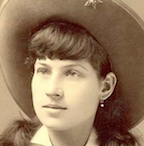
\includegraphics{images/Annie-thumbnail} 

}

\caption{StatPrep Annie}\label{fig:unnamed-chunk-1}
\end{figure}

She's got a website for her course, a couple of interactive lessons, and
so on.

\chapter{Your course web site}\label{your-course-web-site}

As statistics instructors start using data in their classes, they find
that they need to make data files available to students. An excellent
way to do that is to put the files on a web site, so that the students
can access them with a URL.

If your institution uses course support software such as Blackboard or
Moodle, you may want to take advantage of those resources.

Many instructors don't have a web server available to them and aren't
sure how to set up a web site. (And, warranted or not, many instructors
grumble about Blackboard and Moodle) The point of this repository is to
help you set up your own course web site on which you can place data
files, etc. so that your students can easily get to them.

You don't need to know even what a ``repository'' is. You'll be able to
add files to your web site and edit documents from an ordinary brower.

The main resource we'll use is \emph{GitHub}. This is a free service
that's very widely used by software engineers. We won't have to do any
engineering, but you'll have to follow a few instructions.

At this point, make sure that you have a GitHub account. (See
@ref(signing-up-for-cloud-services.html).)

\section{Setting up your web site}\label{setting-up-your-web-site}

\begin{enumerate}
\def\labelenumi{\arabic{enumi}.}
\tightlist
\item
  Open up another browser window, so that you can look at these
  instructions at the same time as you are working on your site.
\item
  Login to GitHub in the browser window you opened in (1).
\item
  Open up one of the following links in the other browser window.

  \begin{itemize}
  \tightlist
  \item
    \href{https://github.com/StatPREP/one-page-website}{One-file web
    site} uses only GitHub.
  \item
    \href{https://github.com/StatPREP/website-template}{Many-file web
    site} requires RStudio for editing. These are both ``repositories''
    under the StatPREP organization.
  \end{itemize}
\item
  Whichever option you selected in (2), find the ``Fork'' button in the
  upper right-hand corner of the StatPREP repository. Chances are,
  you'll be asked whether you want to set this up in your own account.
  You do.
\end{enumerate}

At this point, you should have two browser windows open. One for these
instructions, the other for your GitHub repository. You are going to be
working in the GitHub repository window.

\begin{enumerate}
\def\labelenumi{\arabic{enumi}.}
\setcounter{enumi}{3}
\item
  Press the 
\includegraphics{images/settings-github.png} button. In the
  page that appears \ldots{}

  \begin{enumerate}
  \def\labelenumii{\alph{enumii}.}
  \tightlist
  \item
    Change the name of the repository to something appropriate for your
    course. Stat\_105? Keep it short and don't use any spaces. Use
    underscores instead.
  \item
    Scroll down to the settings section headed GitHub pages.
    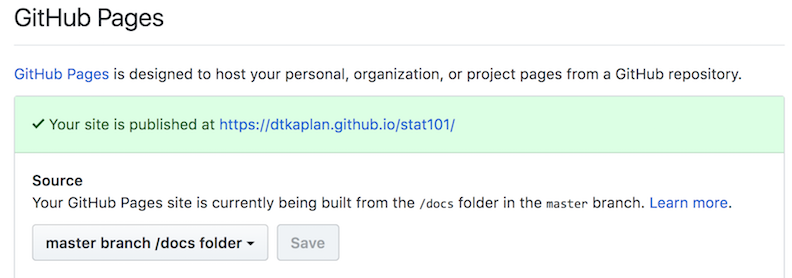
\includegraphics{images/gh-pages.png} Select the drop-down menu to
    read ``master branch /docs folder''.
  \item
    Copy the link that follows ``Your site is published at \ldots{}.''
    This is the link you will give your students. Note that it is formed
    from your GitHub ID and the repository name. That's why you want
    both of these to be memorable.
  \end{enumerate}
\item
  Try it out by pasting the link into the URL bar for another browser
  tab.
\item
  Oh \ldots{} you might want to customize the content before you give
  the link to your students.
\end{enumerate}

\section{Customizing the site
content.}\label{customizing-the-site-content.}

How you are going to customize the content depends on whether you chose
to create a one-page web site or a site that you can edit with RStudio.

\subsection{One-page web site
customization}\label{one-page-web-site-customization}

When you are setting up your repository, you will be logged into GitHub
and at a URL like this:
\texttt{github.com/}\emph{your\_user\_ID}\texttt{/}\emph{your\_course\_name}.

When your students look at the repository, or when you make links to
data files, etc., the URL will look like
\emph{your\_user\_ID}\texttt{.github.io/}\emph{your\_course\_name}. Make
sure it's clear to you how the GitHub user URL differs from the URL for
students.

We're going to do some setup for your site, e.g.~customizing the front
page, adding data files, etc. So check that you are looking at your
GitHub repository:
\texttt{github.com/}\emph{your\_user\_ID}\texttt{/}\emph{your\_course\_name}.

You can see a list of files, starting with a folder called ``docs''. The
docs folder is where you will put all of the materials for your web
site. Click on the name ``docs'' and you will see what files are already
in the directory. There are two:

\begin{itemize}
\tightlist
\item
  \texttt{test.csv} - a really small CSV data file
\item
  \texttt{index.md} - a text file containing the front page of your new
  site.
\end{itemize}

What might confuse you is that the site URL from the students' point of
view is something like
\texttt{http://}\emph{your\_user\_ID}\texttt{.github.io/}\emph{your\_course\_name},
which does not include the word \texttt{docs}. Get used to it. The URL
really does point to the \texttt{docs} directory. And, since there is a
file called \texttt{index.md} in the \texttt{docs} directory, per the
standard behaviour of web sites the contents of \texttt{index.md} are
what will be displayed when someone points their browser to your
\texttt{github.io} site.

Mostly, you're going to do two things with your site:

\begin{enumerate}
\def\labelenumi{\arabic{enumi}.}
\tightlist
\item
  Upload data files from your own computer into the \texttt{docs} folder
  on your site. Conveniently, there is an ``Upload Files'' button just
  for this purpose.
\item
  Edit the \texttt{index.md} file. To do this, click on the name
  \texttt{index.md}, which will open the file. You will see a little
  pencil icon; press that to edit the file. When you're done with your
  edits, scroll down and press the green ``Commit changes'' button. That
  simply saves your work. As soon as you've done this, the modified page
  is live on your web site, but it might take a few minutes and a
  refresh of your browser to see it.
\end{enumerate}

\subsubsection{Putting links to data files on your own course web
site}\label{putting-links-to-data-files-on-your-own-course-web-site}

If you are going to use your site to provide student access to data sets
of particular interest to you, you will want to put links and
instructions on your course web site.

The markup that you include in your \texttt{index.md} file (in the
\texttt{docs/} directory) might look like this:

\begin{verbatim}
## Google files used in class

- `Survey1 <- gs_read(gs_key("1ucevNh7wKLtOukyEpacUKi5_-KZUQGtIOONhWRnnnQ4"))`

## Data files

Data files for this week:

- `https://dtkaplan.github.io/stat101/test.csv`

To create the data table in your R session, copy and paste 
this command into your console:

```r
My_data <- read.csv("https://dtkaplan.github.io/stat101/test.csv")
```
\end{verbatim}

\subsection{Customizing your site with
RStudio}\label{customizing-your-site-with-rstudio}

Outline:

\begin{itemize}
\tightlist
\item
  clone the repo
\item
  open a new project in RStudio, choosing the option for a GitHub
  repository.
\item
  Edit as needed. Every file you edit should be ``knitted'' to HTML.
\item
  State, commit, push, and pull.
\end{itemize}

\chapter{Class data using Google
Sheets}\label{class-data-using-google-sheets}

Collecting data interactively with students has several benefits:

\begin{enumerate}
\def\labelenumi{\arabic{enumi}.}
\tightlist
\item
  Students see the connection between the data and their own actions.
  Students are especially motivated when the data is about them or
  something they are doing.
\item
  The inevitable imperfections in user-entered data serve as a lesson in
  coding factors and the measuring variables in a standard way.
\item
  The instructor (or individual students) can analyze the data and see
  how the analysis changes in real time, as more data rows are added.
\end{enumerate}

\section{Resources}\label{resources}

Two example lessons, from the StatPREP 2018 Workshops are:

\begin{itemize}
\tightlist
\item
  \href{http://dtkaplan.shinyapps.io/tutorial_globe_toss.png}{Globe
  toss}
\item
  \href{http://dtkaplan.shinyapps.io/Tutorial_Riverboat_shuffle.png}{Riverboat
  card trick}
\end{itemize}

You're welcome to use those interactive documents. Each document has a
link to the spreadsheet for entering data. It's your own choice whether
to start by clearing out any existing rows or add on to the rows from
another session. \textbf{NOTE}: No guarantee that your class's data will
be there later on, since someone else might have erased it. And so you
might want to set up your own spreadsheet exclusively for your class's
use.

The section below on \emph{Setting up a new spreadsheet} shows how to
create a spreadsheet for your class. Note that you should post the link
to your spreadsheet on your course website, so that students can access
it to enter data.

For data analysis, you have a choice of options:

\begin{enumerate}
\def\labelenumi{\arabic{enumi}.}
\tightlist
\item
  Use the
  \href{http://dtkaplan.shinyapps.io/Lesson_read_class_data.png}{Read
  class data} activity. The user will have to paste the command to read
  in your spreadsheet at the start of every command block. (See
  \emph{Setting up a new spreadsheet}.)
\item
  Use your own R session. Again, you will need to give the command to
  read in your spreadsheet into the console.
\item
  Create your own tutorial document in Rmd. This presumes that you are
  comfortable editing Rmd documents and, if you want to give your
  students access, publishing them on a server. A working template is
  available via the StatPREP Workshops2018 project on
  \texttt{rstudio.cloud}.
  (\href{https://rstudio.cloud/project/38547}{Follow this link.} to the
  file \texttt{Google\_data\_template.Rmd}.)
\end{enumerate}

\section{Setting up a new
spreadsheet}\label{setting-up-a-new-spreadsheet}

You can modify this document to work with a spreadsheet of your own.
Here's how.

\begin{enumerate}
\def\labelenumi{\arabic{enumi}.}
\item
  Set up a Google spreadsheet. It's a good idea to populate it with some
  variable names and a few values. This will let you test to make things
  are working before you start the activity in class.
\item
  \emph{Within} the Google spreadsheet document press the ``Share''
  button.

  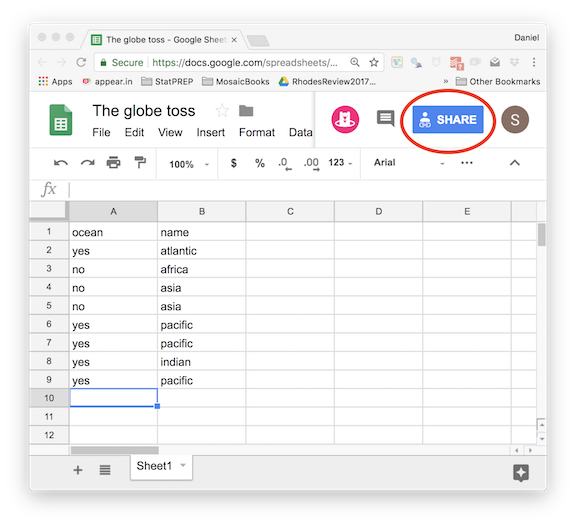
\includegraphics{images/google1.png}
\item
  After you press ``Share,'' you will see a dialog box.

  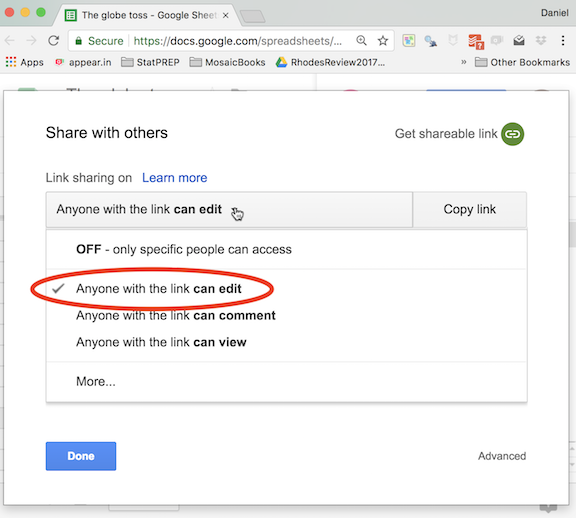
\includegraphics{images/google2.png}

  \begin{itemize}
  \tightlist
  \item
    Pull down the menu to select ``Anyone with the link \textbf{can
    edit}.'' (This is what lets your students add data.)
  \item
    Copy the link and paste it somewhere you can get to it again. You'll
    need it. The link will look like this:
    \texttt{https://docs.google.com/spreadsheets/d/1ucevNh7wKLtOukyEpacUKi5\_-KZUQGtIOONhWRnnnQ4/edit?usp=sharing}
  \item
    You will also need to copy the \emph{key} that's contained in the
    link. The key is just the central gibberish in the link, like this:
    \texttt{1ucevNh7wKLtOukyEpacUKi5\_-KZUQGtIOONhWRnnnQ4}
  \end{itemize}
\item
  Put the link on your course web site so that your students can get to
  it. That's how they will access the spreadsheet for entering data.
\item
  Back in your Google sheet, select the File/Publish\_to\_the\_web menu
  item. Use the resulting dialog box to publish the entire document.
\end{enumerate}

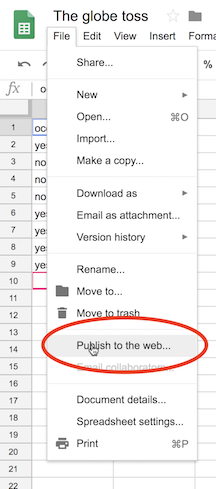
\includegraphics{images/publish1.png}~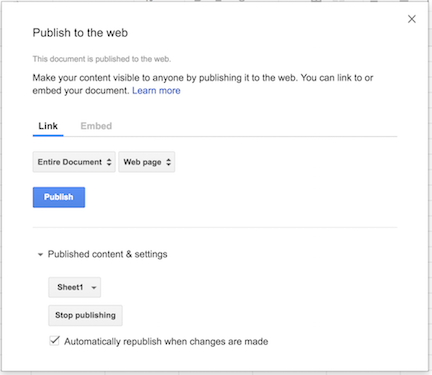
\includegraphics{images/publish2.png}

\begin{enumerate}
\def\labelenumi{\arabic{enumi}.}
\setcounter{enumi}{5}
\item
  Create the R command that will load the spreadsheet data into your R
  session.

\begin{Shaded}
\begin{Highlighting}[]
\NormalTok{Globe <-}\StringTok{ }\KeywordTok{gs_read}\NormalTok{(}\KeywordTok{gs_key}\NormalTok{(}\StringTok{"1ucevNh7wKLtOukyEpacUKi5_-KZUQGtIOONhWRnnnQ4"}\NormalTok{))}
\end{Highlighting}
\end{Shaded}

  In forming the command, replace the quoted string in the above with
  your own key. The key is located in the center of the link to the
  spreadsheet: an incomprehensible set of characters similar to that
  highlighted in \textbf{bold} in the example in step (3). You might
  also replace \texttt{Globe} with a name that's more suited to your own
  activity.

  Paste the command you've created someplace handy. You'll need it.
  (Suggestion: Paste it next to the link in step (4).)
\end{enumerate}

Time for class!

\begin{enumerate}
\def\labelenumi{\arabic{enumi}.}
\setcounter{enumi}{6}
\tightlist
\item
  Once you reach the point in your class where you want to do statistics
  on your data, bring up the lesson document provided for this purpose
  by StatPREP
  \href{http://dtkaplan.shinyapps.io/Lesson_read_class_data.png}{located
  here}. That document has several R command chunks, all of which are
  blank. You can put any R commands in those chunks, \textbf{but make
  sure} that the command from step (5) always is the first command in
  any chunk that you use. That way, whenever you run the code in the
  chunk, the data will be read in from Google. Keep in mind that the
  chunks are all independent of one another, so you'll need to read in
  the data in any chunk you use.
\end{enumerate}

Try it out in the following command chunk:

\begin{enumerate}
\def\labelenumi{\alph{enumi}.}
\tightlist
\item
  Paste in the command you created in step (5).
\item
  Below that, add any R commands you like.
\end{enumerate}

For instructors who want to write their own tutorial, you will find that
this simplifies things since you can arrange to have the spreadsheet
data read-in globally and not have to put the data-reading command in
every chunk. Use the template \texttt{.Rmd} document provided by
StatPREP \href{}{here}. Modify the chunk named \texttt{read\_data} the
top of the document by inserting your own command (with your own key).
Notice that in any new chunk you create, you'll have to reference the
\texttt{read\_data} chunk as the \texttt{exercise-setup}. The chunks
already in the template document do this, so you can just copy (and
rename!) an existing chunk.

\chapter{Using RStudio.cloud}\label{using-rstudio.cloud}

Just some preliminary notes \ldots{}

Under preferences/Rmd, arrange to have the preview opened in the Viewer
tab. It doesn't seem to work to leave it as opening in a web page.

\bibliography{book.bib}


\end{document}
